\PassOptionsToPackage{utf8}{inputenc}
\documentclass{bioinfo}

\copyrightyear{2020} \pubyear{2020}

\access{Advance Access Publication Date: day month 2020}
\appnotes{Application Note}

\usepackage{here}

\begin{document}
\firstpage{1}

\subtitle{Genetic and population analysis}

\title[MPCC]{High Performance Matrix of Pearson$'$s Correlation Coefficient (MPCC) Calculations}
\author[Arends \textit{et~al}.]{
Danny Arends\,$^{\text{\sfb 1, $\dagger$}}$,
Mitch Horton\,$^{\text{\sfb 2, $\dagger$}}$,
Chad Burdyshaw\,$^{\text{\sfb 2, $\dagger$}}$,
Udit Gulati\,$^{\text{\sfb 3}}$,
Christian Fischer\,$^{\text{\sfb 4}}$,
Robert W. Williams\,$^{\text{\sfb 4}}$,
Pjotr Prins\,$^{\text{\sfb 4}}$,
Glenn Brook\,$^{\text{\sfb 2, *}}$}
\address{$^{\text{\sf 1}}$Z{\"u}chtungsbiologie und molekulare
Genetik, Albrecht Daniel Thaer-Institut, Berlin, 10115, Germany \\
$^{\text{\sf 2}}$The Joint Institute for Computational Sciences,
University of Tennessee, Oak
Ridge, TN 37830, USA\\
$^{\text{\sf 3}}$Computer Science Dept. Indian Institute of
Information Technology, Una, Himachal Pradesh, India\\
$^{\text{\sf 4}}$Genetics, Genomics and Informatics, University
of Tennessee Health Science Center, Memphis, TN 38163, USA.}

\corresp{$^\dagger$Contributed equally and should be considered
joined first authors, $^\ast$To whom correspondence should be
addressed.}

\history{Received on XXXXX; revised on XXXXX; accepted on XXXXX}

\editor{Associate Editor: XXXXXXX}

\abstract{ \textbf{Motivation:} With the rapidly
  growing amount of data acquired from sequencing, combined with a
  growing body of phenotype data from medical and experimental
  biology, computing correlations is a recurring
  bottleneck. Especially computation of correlations on incomplete
  data is slow.  Here we present a novel high performance and robust
  matrix-based Pearson correlation coefficent (MPCC) algorithm that
  handles missing data elegantly and makes effective use of modern CPU
  Advanced Vector Extensions (AVX) extensions. \\
\textbf{Results:} Our method is a reformulation of the
  original Pearson's correlation coeffient (PCC) algorithm where
  the lion's share of the computation is handled by fast
  matrix-matrix products. On a single Intel Xeon Gold 6148
  $@$ $2.4$ GHz (Skylake) CPU MPCC achieves 4.3 TFlop/s in single
  precision (i.e., $77\%$ of the theoretical peak). We show how MPCC
  outperforms the existing implementation in R by $200$ times. \\
\textbf{Availability:} Our source code is available as a C
  library for R published under a dual licence, the free and open
  source software GPL-v3 licence as well as the 3-Clause BSD License.
  Source code is available at: \href{https://github.com/UTennessee-JICS/MPCC}{https://github.com/UTennessee-JICS/MPCC}\\
\textbf{Contact:} \href{glenn-brook@tennessee.edu}{glenn-brook@tennessee.edu}\\
\textbf{Supplementary
  information:} Supplementary data are available
  at \textit{Bioinformatics} online.}

\maketitle


\section{Introduction}

The use of Pearson's correlation coefficient (PCC) is ubiquitous
across all fields of biology ranging from agriculture to
zoology. Large scale computation of correlations are found in many
areas of biology and bioinformatics.  For example, genotype
correlations are used to construct haplotypes, build genetic maps, and
order markers within the genome. Pearson's correlations are also used
in co-expression analysis \citep{Tesson:2010}, (genome wide)
association analysis, reconstruction of genetic
networks \citep{Fukushima:2013}, weighted correlation network analysis
(WGCNA) \citep{Horvath:2008} and correlated trait locus (CTL)
mapping \citep{Arends2016a}.


%The mathematical formula for Pearson$'$s correlation were derived by
%Auguste Bravais in 1844. However, as Stigler's Law \citep{Stigler1980} dictates,
%the name of the method credits Karl Pearson, who was building on ideas published
%by Francis Galton in the 1880s.

\enlargethispage{12pt}

The work presented here is motivated by Genenetwork, a service for
web-based genetics \citep{Sloan2016} which routinely performs a matrix
of Pearson's Correlation Coefficient (PCC) calculations to find
relationships between and among genotypes and phenotypes in mouse and
rat strains. These calculations are a bottleneck for moderate to large
problem sizes.

% , especially when accounting for missing data.


Consider the case where correlation is computed within a set of
phenotypes. The BxD family is a panel of 150 recombinant inbred mice
derived from parents C57BL/6J and DBA/2J \citep{Ashbrook:2019}. The
BxD data collection in Genenetwork consists of high-density genotypes
with 7,000 classical phenotypes and several data sets containing
100,000+ gene expression phenotypes. Statistics are often computed in
the R language for statistical computing \citep{R:2005}. R's default
$cor()$ implementation of Pearson's correlation is pairwise and
written in C and is especially slow when accounting for missing
data. Simply removing individuals with missing phenotype or genotype
data does not work here because most studies use different subsets of
these 150 mice. A matrix-style correlation computation based on
removing rows with missing phenotypes would therefore end up being
empty.  With MPCC we implemented a novel matrix based approach, that
is a drop-in replacement for $cor()$ and can handle missing data
without loss of performance.

\begin{figure}[H]
\centering
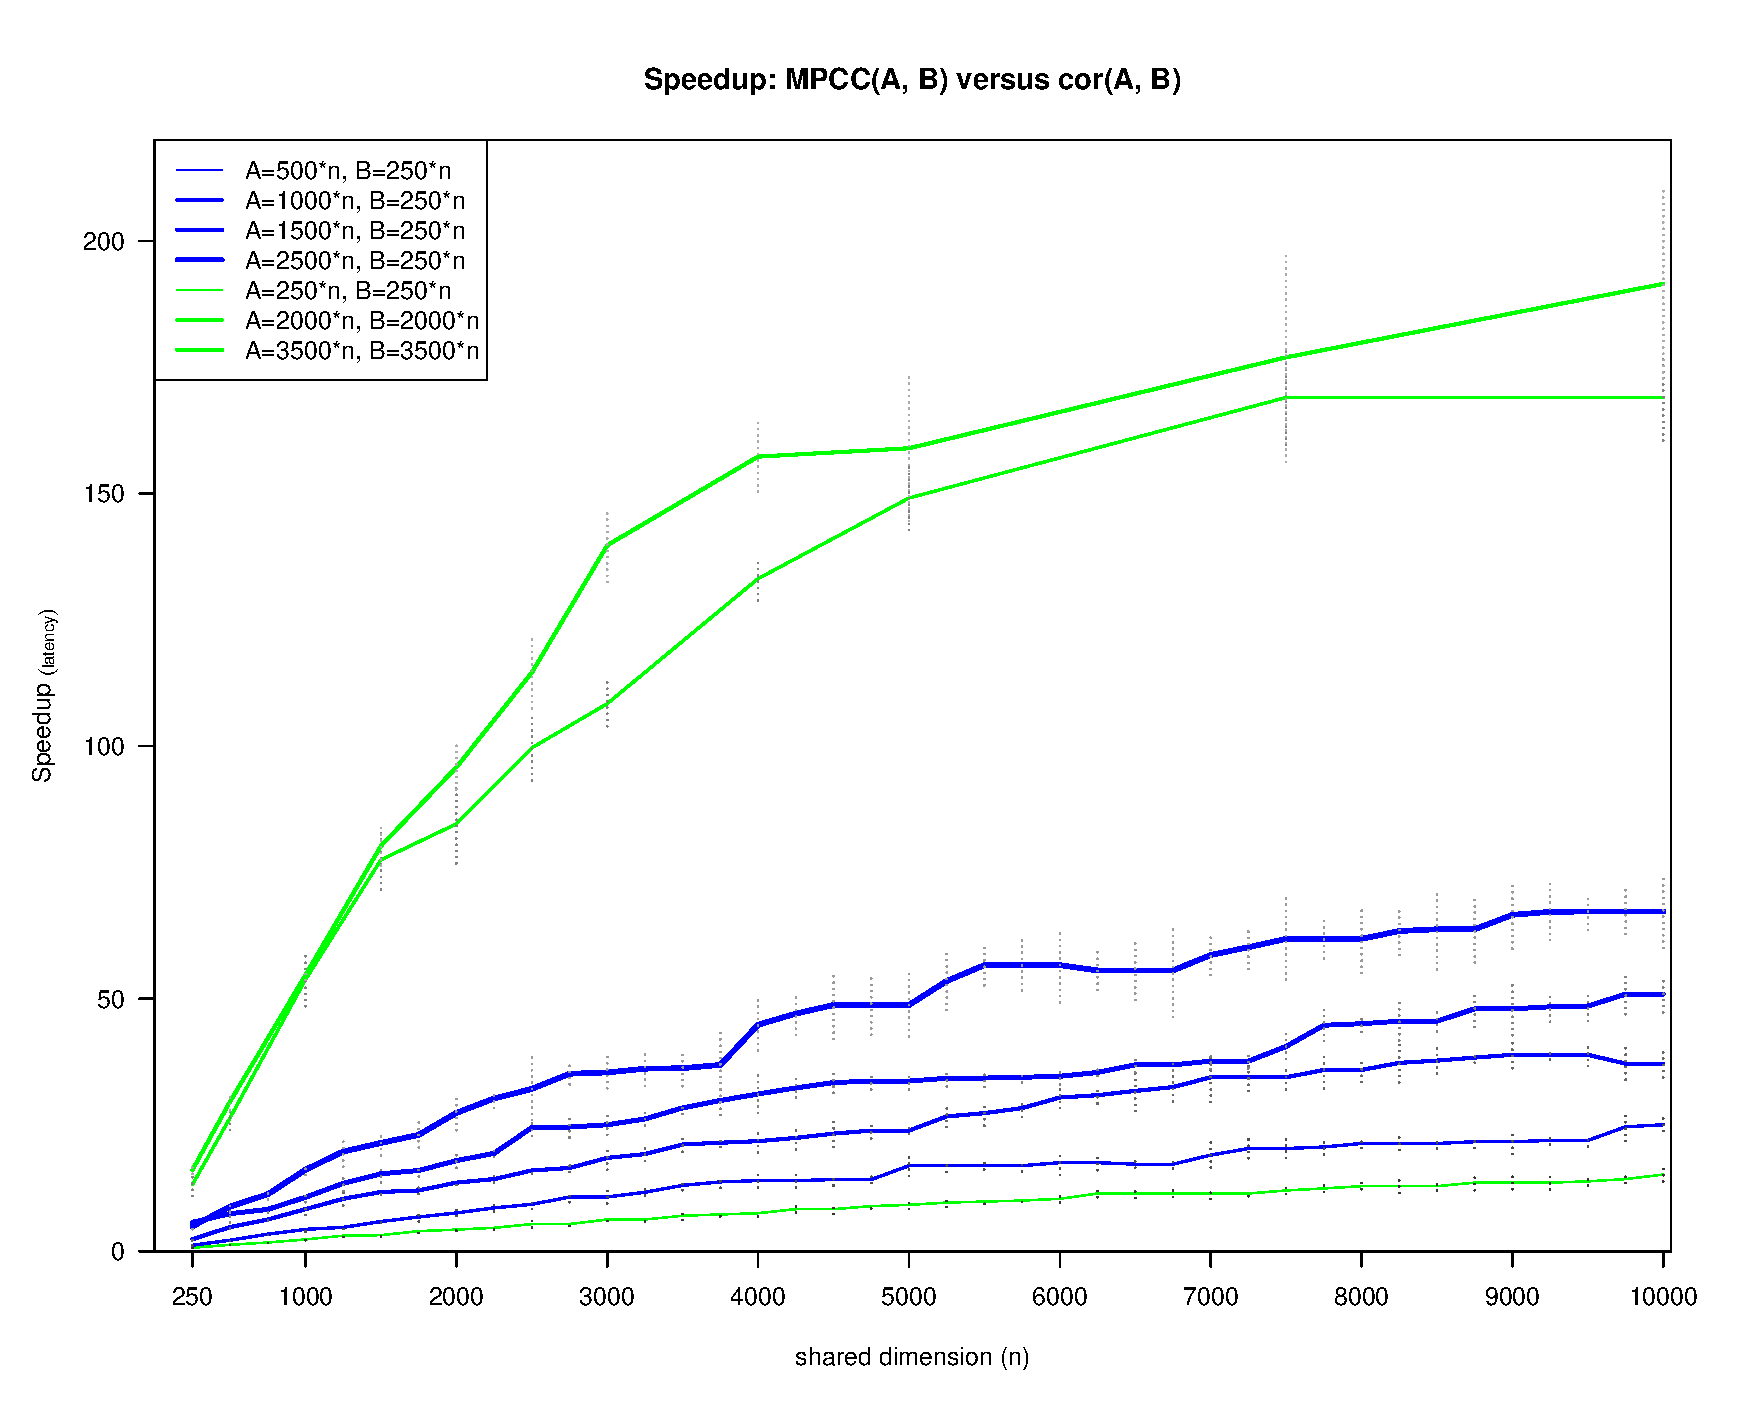
\includegraphics[width=\linewidth]{img/figure02new.eps}
  \caption{ \small Speed comparison of MPCC versus the native R $cor$
  function shows increased performance with increased matrix
  sizes. Square matrices (green) run faster than the non-square
  matrices (blue).  The effect of handling missing data (0 to 50\%) is
  visualized with error bars - i.e. these show that missing data
  handled by MPCC bit-masking has limited effect on performance.
  Multi-threaded performance for a 3500x3500 matrix shows a potential
  200$\times$ speedup compared to the default $cor()$ function.  All
  timings were performed on a system with 28 cores (56 hyper threaded)
  Intel(R) Xeon(R) CPU E5-2680 v4 @ 2.40GHz.  } \label{fig:fig2}
\end{figure}

\vspace*{-10mm}

%  MPCC always performs missing data Bit-masking, while the R
%  $cor()$ function suffers from increased runtime with increasing
%  amount of missing data.

\section{Approach}

We started work on optimizing the speedup of correlations by writing a
version that is algorithmically identical to the R $cor()$ function
(see supplement). Next, we added multi-threading by introducing
OpenMP. This provided a limited speedup, typically in the order of
3.5$\times$ compared to the single core version.  Next, we wrote MPCC,
a matrix implementation of Pearson's correlation that makes effective
use of hardware Advanced Vector Extensions (AVX) instructions
introduced by Intel in 2011. This approach sped up computations up to
$200\times$ on a 28-core machine (Figure~\ref{fig:fig2}).  The MPCC
matrix version reformulates the original algorithm into a series of
matrix-matrix products and element-wise matrix operations. MPCC
handles missing data by using a novel bit-masking approach that
leverages existing matrix-matrix multiplication implementations from,
for example, OpenBLAS (Supplement 1 - 'Missing Data Bit-masking').
MPCC leverages the optimized speed of OpenBLAS or, alternatively,
Intel\textregistered{} MKL, to obtain maximum performance on systems
that support the AVX instruction sets.

To benchmark MPCC for different matrix sizes we computed pairwise
correlation between genotypes of the BxD family.  Genotype data in the
BxD family is complete with only a few heterozygous or `missing' loci
remaining, i.e., it benchmarks MPCC versus $cor()$ when a small amount
of data is missing.  Next we computed the speed improvement of MPCC
versus R's $cor()$ for these matrices. We increased step-wise the
amount of missing data by masking genotypes. Even on a single core
MPCC showed a
\textasciitilde{}$5\times$ speedup compared to the $cor()$
function provided in R. With multi-threading MPCC
gains with every core added, up to $200\times$ (Figure \ref{fig:fig2}).

MPCC is written in C$++$, and provides a C foreign function interface.
The algorithm can therefore be called from any other computer language
using a foreign function interface. Our work presents such a binding
in the R programming language, providing other researchers with
an example on how-to call the MPCC algorithm from other programming languages.

\vspace*{2mm}
\section{Discussion}

MPCC is a matrix based computational reimplementation of the original
correlation algorithm. MPCC makes use of multi-threading and modern
vector extensions of the CPU hardware.  The bit-masking missing data
approach can be generalized to other algorithms which rely on
matrix-matrix multiplication and may also be suitable for GPU
computing.

With this work we not only introduce a faster routine that reduces
regularly occurring bottlenecks in large correlation computations, but
also we show that it can pay off to revisit 'obvious' implementations
of routines in common use today that were written over 20 years
ago. Computer hardware and architecture is still changing and
dedicated optimization work may benefit both interactivity for
end-users and large scale computations on high perfomance compute
clusters at the same time.


\section*{Funding}

We thank the support of Xsede/NSF startup MCB190140, the UT Center for
Integrative and Translational Genomics, and funds from the UT-ORNL
Governor's Chair, NIGMS Systems Genetics and Precision Medicine
Project R01 GM123489, NIDA grant P30 DA044223, NIAAA U01 AA013499 and
U01 AA016662.\\
\textit{Conflict of Interest:} none declared.

\vspace*{-5mm}
\bibliographystyle{natbib}
\bibliography{main}

\end{document}
